\documentclass{tufte-handout}
\title{Sensitivity Calculations}
\author[mohamedkamal]{Mohamed Kamal Abd Elrahman \\
6 October, Giza,\\ Egypt}

\usepackage{amsmath}  % extended mathematics
\usepackage{svg}

\usepackage{graphicx} % allow embedded images
\setkeys{Gin}{width=\linewidth,totalheight=\textheight,keepaspectratio}
\graphicspath{{graphics/}} % set of paths to search for images
\usepackage{amsmath}  % extended mathematics
\usepackage{booktabs} % book-quality tables
\usepackage{units}    % non-stacked fractions and better unit spacing
\usepackage{multicol} % multiple column layout facilities
\usepackage{lipsum}   % filler text
\usepackage{fancyvrb} % extended verbatim environments
\fvset{fontsize=10}% default font size for fancy-verbatim environments

% Standardize command font styles and environments
\newcommand{\doccmd}[1]{\texttt{\textbackslash#1}}% command name -- adds backslash automatically
\newcommand{\docopt}[1]{\ensuremath{\langle}\textrm{\textit{#1}}\ensuremath{\rangle}}% optional command argument
\newcommand{\docarg}[1]{\textrm{\textit{#1}}}% (required) command argument
\newcommand{\docenv}[1]{\textsf{#1}}% environment name
\newcommand{\docpkg}[1]{\texttt{#1}}% package name
\newcommand{\doccls}[1]{\texttt{#1}}% document class name
\newcommand{\docclsopt}[1]{\texttt{#1}}% document class option name
\newenvironment{docspec}{\begin{quote}\noindent}{\end{quote}}% command specification environment

\begin{document}
	\maketitle
	\begin{abstract}
		\noindent 
	Sensitivities are used as measures of robustness for engineering systems. In many applications, one is interested about the system performance under small variations of a set of design parameters. In inverse device design, sensitivities guides the search within the space spanned by a set of design parameters. 
	\end{abstract}
\section{Problem Formulation}	
 Assuming $\mathbf{G}$	is a vector of design merits $ (G_1[\mathbf{x}], G_2[\mathbf{x}], \dots,G_n[\mathbf{x}]) $, where each component is a scaler function of $m$ design parameters $\mathbf{x}$	$ (x_1,x_2,\dots, x_m)$. The goal is to find the sensitivity of the design merit $G_i$  with respect to the design parameter $x_j$:
	 \begin{equation}
	 S_{ij} = \frac{d G_i}{dx_j}
	 \end{equation}
The entries $S_{ij}$ form the elements of the  $n \times m$  Jacobian matrix $S$ which maps $m$ input parameters to $n$ output merits.   The Jacobian could be seen as a generalization of the slope constant $s$ in $g(x) = s x$, but now is used for multivariate vetor functions. The entries of row $S_i = \frac{d G_i}{d \mathbf{x}}$ are the sensitivities of the merit function $G_i$ with respect to all the design parameters. The entries of column $S_j = \frac{d \mathbf{G}}{d x_j}$ are the sensitivities of all the merit functions with respect to the single design parameter $x_j$

%\section{Symbolic Differentiation}  

\section{Finite Difference Method}
In the finite difference approximation, the sensitivity column $\frac{d \mathbf{G}}{dx_j}$  is calculated by perturbing the design parameter $x_j$  by a step $\Delta x_j$ and then evaluating the new merits $\mathbf{G}$.  In its simplest form, it is based on the limit definition of a derivative:
\begin{equation}
\frac{d \mathbf{G}}{dx_j} \approx  \frac{\mathbf{G}(\mathbf{x} + \mathbf{\Delta}_j) - \mathbf{G}(\mathbf{x})}{\Delta_j}
\end{equation}
where $\mathbf{\Delta}_j = \Delta_j {\mathbf{\hat{e}}_j}$.
If we have $m$ design parameters, we need to finite difference $m$ times to fill all the columns of the Jacobian $S$.The finite difference is simple to implement, but there are  some severe disadvantages: 
\begin{itemize}
	\item The objective function  may be very costly to be perturbed and evaluated $m$ times, especially if $m$ is large.
	\item The finite difference suffers from truncation errors \sidenote[1]{Truncation error is the error of approximation, or inaccuracy, one gets from h not actually being zero. It is proportional to a power of $\Delta$.} \sidenote[2][.5\linewidth]{Finite difference approximation commits both cardinal sins
		of numerical analysis: "thou shalt not add small numbers to big numbers", and "thou shalt not subtract numbers which are approximately equal"} so the step size $\Delta_j$  should be very  small. Practically, a very small step will lead to subtractive cancellation errors . So choosing a balanced step size is a problem by itself and we need to solve the this problem $m$ times for each design parameter. 

	
	\begin{figure}[h]
		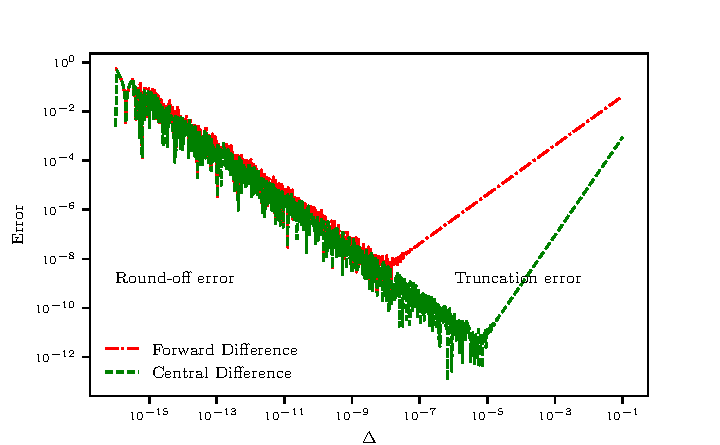
\includegraphics[width=\linewidth]{fd_error_types.pdf}%
		\caption{Error in the forward  and central difference approximations as a function of step size $\Delta$.}%
		\label{fig:fullfig}%
	\end{figure}

	
\end{itemize}
 The numerical accuracy could be improved by using higher-order finite differences , however it also   increased computational complexity and did not not completely eliminated truncation errors.
\section{Automatic Differentiation}
 Automatic differentiation (AD), also called algorithmic differentiation, is a family of techniques for efficiently and accurately evaluating derivatives of numeric functions expressed as computer programs. The key idea behind AD is  that all complicated mathematical functions will be at the end represented on a computer by a composition of a finite set of elementary operations $(+,-,/,*,\sin,\cos,\sqrt )$  with exactly known partial derivatives.  Chain rules would then be applied to find the overall derivatives. Automatic differentiation comes in two modes, the forward mode and the reverse mode.  The reverse mode is advantageous for calculating the sensitivities of a small number of outputs with respect to a large number of input parameters. The forward mode is advantageous in the opposite case, when the number of outputs is larger compared to the number of inputs.
 %The best way to see this is by example.
 %\subsection{Example}



%\subsection{Automatic Forward-Mode Differentiation}
%\subsection{Automatic Reverse-Mode Differentiation}

\end{document}